\documentclass[../../main]{subfiles}
\begin{document}
\newpage
\subsection{Live events}
\label{ss:final-live}
A live events is a special poi that has a certain time to live specified during the creation. They are build to be always public and to notify 
all user's friends when he creates one. The differents of the details dialog from a live event and a poi are that on a live event, instead of showing 
the url and website, are listed the expiration date and the owner of the live event. The image below show the dialog of the creation of a live event and the dialog of details about a live event.
\begin{figure}[H]
    \centering
    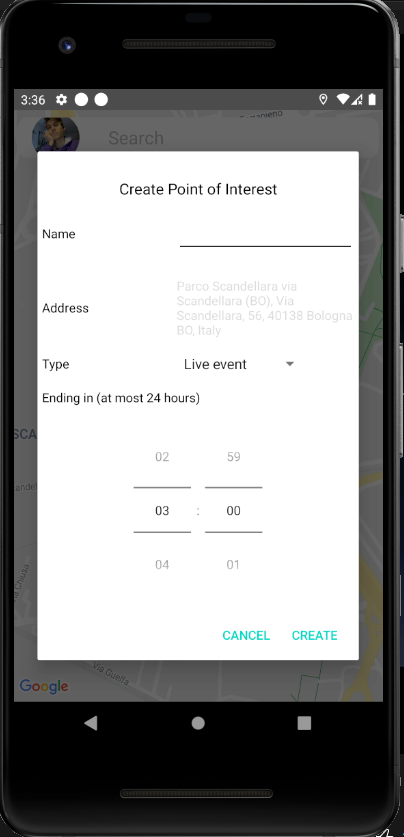
\includegraphics[width=70mm,height=150mm]{images/app/live/creazione_live.png}
    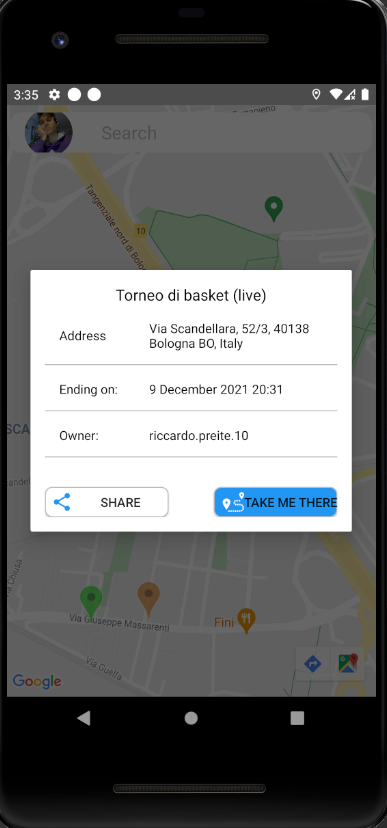
\includegraphics[width=70mm,height=150mm]{images/app/live/live_map_detail.png}
    \caption{On the left the dialog to create a live event with the timer and on the right the dialog of details about a live event.}
\end{figure}

As said in \ref{ss:final-friends} a user is notified when one of his friend add a live event but he can also see all the poi currently active by navigating
to the apposite live list on the main menu fragment.
\begin{figure}[H]
    \centering
    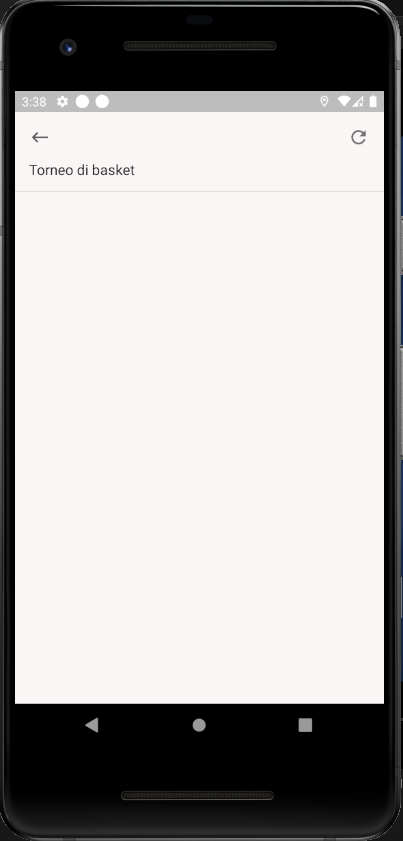
\includegraphics[width=70mm,height=150mm]{images/app/live/live_overview.png}
    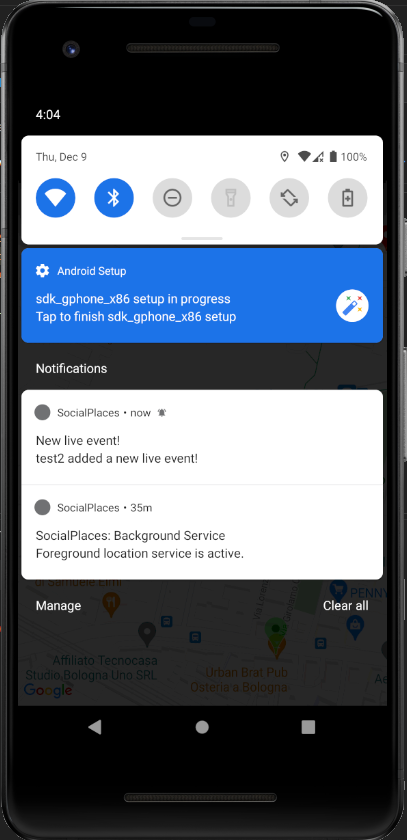
\includegraphics[width=70mm,height=150mm]{images/app/notification/live/notifed_live.png}
    \caption{On the left the list of live events active and on the right the notification of a new live event added.}
\end{figure}
\end{document}